\documentclass{article}
%\usepackage[a4paper, total={6in, 8in}]{geometry}
\usepackage{geometry}
\usepackage{lipsum}
\usepackage{mwe}
 \geometry{
 a4paper,
 total={210mm,297mm},
 left=20mm,
 right=20mm,
 top=-2mm,
 bottom=2mm,
 }
%\usepackage[margin=0.5in]{geometry}

\usepackage{amsmath,amssymb}
\usepackage{ifpdf}
%\usepackage{cite}
\usepackage{algorithmic}
\usepackage{array}
\usepackage{mdwmath}
\usepackage{pdfpages}
\usepackage{mdwtab}
\usepackage{eqparbox}
\usepackage{cite}
%\onecolumn
%\input{psfig}
\usepackage{color}
\usepackage{graphicx}
\setlength{\textheight}{23.5cm} \setlength{\topmargin}{-1.05cm}
\setlength{\textwidth}{6.5in} \setlength{\oddsidemargin}{-0.5cm}
\renewcommand{\baselinestretch}{1}
\pagenumbering{arabic}
\usepackage{ragged2e}
\renewcommand{\baselinestretch}{1.5}

\begin{document}

\textbf{
\begin{center}
{
\large{School of Engineering and Applied Science (SEAS), Ahmedabad University}\vspace{4mm}
}
\end{center}
%
\begin{center}
\large{B.Tech(ICT) Semester V: Wireless Communication (CSP 311) }\\ \vspace{3mm}
\end{center}
}
\begin{itemize}
\item Group No : G4Vcps
\item Name (Roll No) : \newline Priyanshi Deliwala(AU1741047) \newline Nimil Shah(AU1741048) \newline Aayushi Ganatra(AU1741050) \newline Shashwat Mehta(AU1741100)%\item Roll no: s1749002 (Ph.d)
%\item Associated with Project: DST-UKIERI
\item Project Title:
\subitem 1) Performance analysis of vehicle-to-vehicle communication with full duplex amplify-and-forward relay over double-Rayleigh fading channels
\subitem 2) Performance analysis of vehicle-to-vehicle communication with full duplex amplify-and-forward relay over double-Rayleigh fading channels with multiple antennas on Relay Node(SIMO MISO Double Rayleigh Fading)
\end{itemize} 

\section{Introduction}
\subsection{Background}
.
\begin{itemize}
    \item Spectrum is everything with regards to picking or structuring remote hardware.In the age of digital technology almost all personal devices are connected to the internet to exchange data. However in past few years the users have increased significantly therefore creating the issue of limited available spectrums. 
    \\Today, vehicular communications assume a significant job because of their applications in self-governing vehicles In addition, nearly individuals control the framework through the  gadgets in any event, when these gadgets proceed onward the street, which structure the  (V2V) correspondence.
    \\Since the diverts between the gadgets in V2V correspondence show double Rayleigh fading, they are more terrible than the directs in conventional remote communications where the channels between the gadgets are generally portrayed by Rayleigh fading. Subsequently, the framework execution of V2V will be diminished in examination with that of customary remote correspondence
    
    \item FD communication has become the most favourable solution to the issue of Wireless spectrum. With the development of antenna design techniques, FD devices can suppress the SIC. Moreover on using a relay node reliability, coverage and performance of Wireless Systems is improved. This way FD systems can nearly double the usage of spectrums.
    
    
      
\end{itemize}

\subsection{Motivation}
We observe that there is a lack of research on FD-V2V communications systems because when FD and V2V communication systems are combined the system performance will be decreased due to Double Rayleigh Fading. Motivated by this issue we can combine different system models with FD V2V and compare the results with Double Rayleigh Fading.

\subsection{Contributions}
\begin{itemize}
Contribution-1 \\
\item   Symbol Error Rate Contribution:\\
\item An important reference for the analysis  of any modulation scheme is the Symbol Error rate(SER) for the corresponding system model. The closed form expressions for BPSK modulation has been mentioned in the report for analytical results.
\\The results have been derived for transmission of symbols transferred for different scenarios such as : Different Path Loss exponents, Same and different distances between mobile nodes, different SNRs etc.However, even though relay node worked as a AF full duplex relay node, SER was not being decreased significantly. Later it was inferred that since when relay works as a transmitter the signal which has been received on the single antenna can be only send.
\\Therefore if the number of antennas are increased on the relay node different signal can be received by different antennas and the signal with highest signal strength can be transmitted using AF protocol 
 \\\\Contribution-2 
 \item
\\\\ The Outage Probability of the considered system is defined as the probability that the transmission rate of the system is less than the a given data rate.
\\The closed form for the Outage Probability has been mentioned in the report where SINR is calculated for the fixed and variable gain. We investigated the the OPs for the FD-V2V communication system for the respective gains. Demonstrated how the performance is degraded over Double-Rayleigh fading channel. Further, we extended this work by analyzing the scenario where the respective system model is varied for V2V communication systems.
\item
\\\\ The Throughput of the considered system can be defined as a function of Outage Probability. In Outage Probability, we define $\gamma$ as the SINR for Fixed and Variable Gain for the FD-V2V communication system.
\\Hence, we characterize $\gamma_{0}$ as the Threshold of the Outage Probability which then equates to,
$P_{out} = Pr(\gamma < \gamma_{0})$
\\From this, we derive the function of Throughput as follows :
$\gamma_{0} = 2^{R} - 1$
\\where, R is the Minimum Data Rate required.


\end{itemize}

%are Once accomplished,we can improve sensing performance based on  the knowledge of channel statistics. Further, for more realistic considerations we would extend the above setup to SIMO, MISO and MIMO system models. The performance metrics would be the statistical properties like idle/busy period durations, its mean, variance and Occupancy rate(or duty cycle) of Primary user (PU). The metric for spectrum sensing would be detection probability $(P_d).$ Also the estimation error varies as per sensing period$(T_s)$ and thus KS distance would be an additional metric to be taken into consideration. 
	%\vspace{8cm}
\section {Performance Analysis of Base Article}
\begin{itemize}
\item List of symbols and their description

\begin{table}[]
 \centering
 \caption{List of notations used}
 
 \begin{tabular}{|c|c|}
 \hline
 \textbf{Symbol} & \textbf{Description}                                                                                           \\ \hline
$ y_{D}$          & Received Signal at Destination                                                                                       \\ \hline
 $ y_{R}$        & Received Signal at Receiver                                                                                     \\ \hline
 $\gamma_{RSI} $       & Variance of Gaussian Distribution                                                                                                                                                        \\ \hline
 $G_{f} $       & Fixed Gain corresponding to the channel condition                                                                                                                                                       \\ \hline
 $G_{v} $       & Variable Gain corresponding to the channel condition                                                                                                                                                           \\ \hline 
  $(g_{1}, g_{2}) $       & Independent Rayleigh Variable   
                                                                    \\ \hline
    $\rho_{1},\rho_{2} $       & Instantaneous channel gains                                                                                                                                      \\ \hline
    $\gamma_{0} $       & Threshold of the Outage Probability  
                                                                    \\ \hline
                                                                    
    $P_{out} $       & Outage Probability of the considered system                                                                                                                                                       \\ \hline
    $\Omega_{1},\Omega_{2} $       & Average channel gains of links, respectively                                                                                                                                      \\ \hline
    $K_{0},K_{1} $       & Zero and First-Order modified Bessel Functions                                                                                                                                      \\ \hline
    $P_{out}^{f} $       & Fixed Gain Outage Probability                                                                                                                                                       \\ \hline
    $P_{out}^{v} $       & Variable Gain Outage Probability                                                                                                                 \\ \hline
    $SER$       & Symbol Error Rate                                                                                                                 \\ \hline
    $SER_{v}$       & Fixed Gain Symbol Error Rate                                                                                                                 \\ \hline
    $SER_{f}$       & Variable Gain Symbol Error Rate                                                                                                                 \\ \hline
  
 %$G_{f}$             & \begin{tabular}[c]{@{}c@{}}Number of sensing events 
 %\end{tabular}                                                                      \\ \hline
 \end{tabular}
 \end{table}





\item System Model/Network Model : 
$y_R= \sqrt{d_SR^-\alphaP_S}h_SRx_S + I_R + n_R$
As illustrated in Fig the signal is transmitted from a source node(S) to a destination node(D) via a relay R. Two separate antennas are used on relay node for transmission and receive to implement FD. $h_{SR}$ and hrs are the channel coefficients for Double Rayleigh fading and $n_{R}$ is the Additive White Gaussian Noise.
\begin{center}
\includegraphics[height=6cm] {SYSTEMMODEL.PNG}
\begin{figure}[h!]
    
    \label{fig:}
\end{figure}
\end{center}





\item Detailed derivation of performance metric-I
\\\\Outage Probability :
\\\\Firstly, we would start with the Rayleigh fading channel.
\\The probability density function (PDF) and cumulative distribution function
(CDF) of its instantaneous channel gain $\rho = |g|^{2}$ are respectively
given by $f_{\rho}(x)$ = $\frac{1}{\Omega} exp (-\frac{x}{\Omega})$
\\\\$F_{\rho}(x)$ = $1 - exp (-\frac{x}{\Omega})$
\\where $\Omega = E(\rho)$

\\\\Now here,
\\For the Double Rayleigh fading channel in V2V communication, its instantaneous channel gain $|h|^{2}$ can be characterized as follows :
\\The multiplication of two independent variables $|g_{1}|^{2}$ and $|g_{2}|^{2}$, i.e. $|h|^{2}$ = $|g_{1}|^{2} |g_{2}|^{2}$ = $\rho_{1}\rho_{2}$, where $|g|_{1}^{2}$ and $|g_{2}|^{2}$ are the instantaneous channel gains of the Rayleigh fading channels.
\\Hence, due to the fact that $\rho_{1}$ and $\rho_{2}$ are independent variables, we have the CDF of $|h|^{2}$ as,
\\\\$f_{|h|^{2}}(x)$ = $Pr(\rho_{1}\rho_{2}\leq x)$
\\\\ = $\int_{0}^{\infty} Pr(\rho_{2}\leq \frac{x}{\rho_{1}})f_{\rho_{1}}(y)dy$
\\\\$1 - \frac{1}{\Omega_{1}} \int_{0}^{\infty} exp(-\frac{y}{\Omega_{1}}-\frac{x}{y\Omega_{2}})dy$
\\\\$1 - \sqrt{\frac{4x}{\Omega_{1}\Omega_{2}}}K_{1}(\sqrt{\frac{4x}{\Omega_{1}\Omega_{2}}})$\\

\\\\We would now obtain the PDF of $|h|^{2}$ as follows :
\\\\$f_{|h|^{2}}(x) = \frac{2}{\Omega_{1}\Omega_{2}}K_{0}(\sqrt{\frac{4x}{\Omega_{1}\Omega_{2}}})$
\\\\where $\Omega_{1}$ = E$(\rho_{1})$, $\Omega_{2}$ = E$(\rho_{2})$

\\\\Therefore now, we derive the expressions for the Fixed Gain Outage Probability and Variable Gain Outage Probability,


\\$Pr(\gamma_{f}<\gamma_{0})$
\\\\ = $Pr(\frac{(d_{SR}d_{RD})^{-\alpha}P_{S}P_{R}X Y}{d_{RD}^{-\alpha}P_{R} Y (\gamma_{RSI}+\sigma^{2})+\frac{\sigma^{2}}{G_{f}^{2}}} \leq \gamma_{0})$

\\\\$Pr(\gamma_{v}<\gamma_{0})$
\\\\ = $Pr(\frac{(d_{SR}d_{RD})^{-\alpha}P_{S}P_{R}X Y}{d_{RD}^{-\alpha}P_{R} Y (\gamma_{RSI}+\sigma^{2})+ \sigma^{2}(d_{SR}^{-\alpha}P_{S}X + \gamma_{RSI} + \sigma^{2})} \leq \gamma_{0})$
\\where $X = \rho_{1\rho_{2}}$ ; $Y = \rho_{3}\rho_{4}$
\\\\Here, as we combine the PDF and the CDF of the instantaneous channel gain of double Rayleigh fading channel, we can calculate $P_{out}_{f}$ and $P_{out}^{v}$ as follows : 
\\\\$P_{out}^{f} = Pr(\frac{(d_{SR}d_{RD})^{-\alpha}}P_{S}P_{R}XY{d_{RD}P_{R}Y(\gamma_{RSI} + \sigma^{2}) + \frac{\sigma^{2}}{G_{f}^{2}}} \leq \gamma_{0})$
\\\\ = $Pr(X<\frac{\sigma^{2}\gamma_{0}}{G_{f}^{2}(d_{SR}d_{RD})^{-\alpha}P_{S}P_{R}Y} + \frac{(\gamma_{RSI} + \sigma^{2})\gamma_{0}}{d_{SR}^{-\alpha}P_{S}})$
\\\\ = $1 - \int_{0}^{\infty}[1 - F_{x}(\frac{\sigma^{2}\gamma_{0}}{G_{f}^{2}(d_{SR}d_{RD})^{-\alpha}P_{S}P_{R}\xi} + \frac{(\gamma_{RSI} + \sigma^{2})\gamma_{0}}{d_{SR}^{-\alpha}P_{S}})]f_{Y}(\xi)d\xi$
\\
\\\\We see here that, since X and Y are the instantaneous channel gains of double Rayleigh fading channels, the PDF and CDF of X and Y have already been mentioned above.
\\Therefore, the $P_{out}^{f}$ is calculated as,
\\\\$P_{out}^{f}$ = $1 - \int_{0}^{\infty}\sqrt{\frac{4 \sigma^{2}\gamma_{0}}{\Omega_{1}\Omega_{2}G_{f}^{2}(d_{SR}d_{RD})^{-\alpha}P_{S}P_{R}\xi} + \frac{4(\gamma_{RSI} + \sigma^{2})\gamma_{0}}{\Omega_{1}\Omega_{2}d_{SR}^{-\alpha}P_{S}}}$ X $ K_{1}(\sqrt{\frac{4\sigma^{2}\gamma_{0}}{\Omega_{1}\Omega_{2}G_{f}^{2}(d_{SR}d_{RD})^{-\alpha}P_{S}P_{R}\xi} + \frac{4(\gamma_{RSI} + \sigma^{2})\gamma_{0}}{\Omega_{1}\Omega_{2}d_{SR}^{-\alpha}P_{S}}})$ X \\$\frac{2}{\Omega_{3}\Omega_{4}}K_{0}(\sqrt{\frac{4\xi}{\Omega_{3}\Omega_{4}}})d\xi$
\\\\ $ = C_{f} \int_{0}^{\infty} \sqrt{\frac{A_{f}\gamma_{0}}{\xi} + B_{0}\gamma_{0}} K_{1} (\sqrt{\frac{A_{f}\gamma_{0}}{\xi} + B_{f}\gamma_{0}})$ X $ K_{0} (\sqrt{2C_{f}\xi})d\xi$
\\
\\Finally, by setting $\nu = e^{-\xi}$, the above equation can be rewritten as follows : 
\\$P_{out}^{f} = 1 - C_{f} \int_{0}^{1} \sqrt{\frac{A_{f}\gamma_{0}}{-ln\nu} + B_{f}\gamma_{0}K_{1} (\sqrt{\frac{A_{f}\gamma_{0}}{-ln\nu}} + B_{f}\gamma_{0})}$ X $K_{0} (\sqrt{-2C_{f}ln\nu})\frac{d\nu}{\nu}$

\\\\Since X and Y are the instantaneous channel gains of double
Rayleigh fading channels, the PDF and CDF of X and Y are given
above respectively. Therefore, the Pv out is calculated as,
\\\\For the $P_{out}^{v}$, we have,


\\$Pr(\gamma_{v}<\gamma_{0})$
\\\\ = $Pr(\frac{(d_{SR}d_{RD})^{-\alpha}P_{S}P_{R}X Y}{d_{RD}^{-\alpha}P_{R} Y (\gamma_{RSI}+\sigma^{2})+{\sigma^{2}}({ d_{SR}^{-\alpha}P_{S} X + \gamma_{RSI}+\sigma^{2}})}) \leq \gamma_{0})$
\\\\
= $P_r\{d^{-\alpha}_{SR} X P_S(d^{-\alpha}_{RD} P_RY -\sigma^{2} \gamma_0) < d^{-\alpha}_{RD} P_R Y(\gamma_{RSI} + \sigma^{2})\gamma_0 +( \gamma_{RSI} + \sigma^{2}) \sigma^{2}\gamma_0\}$
\\
\\ Then, by setting Y = Z + $\frac{\sigma_{2}\gamma_0}{d_{RD}-\alpha}$, becomes



\\\\$P_{out}^{v} =
P_r\{(d_{SR}d_{RD})^{-\alpha} P_S P_R X Z < d_{RD}P_R (Z + \frac{\sigma_{2}\gama_0}{d_{RD}^{-\alpha} P_R}$)  
         (\gamma_{RSI} + \sigma_{2})\gamma_0 +  (\gamma_{RSI} + \sigma_{2})\sigma_{2}\gamma_0\} 
\\\\$We can calculate the $P_{out}^{v}$ out by using the same method as for$P_{out}^{f}$, i.e.,$

\\\\\\\\$P_{out}^{v}$ = \int_{0}^{\infty}[$1 - F_x(\frac{(\gamma_{RSI}+ \sigma_{2})\sigma^{2}(\gamma_{0} + \gamma^{2})}{(d_{SR}d_{RD})^{-\alpha} P_S P_R \xi} + \frac{(\gamma_{RSI} + \sigma^{2}) \gamma_0}{d_{SR}^{-\alpha} P_S})] f_z(\xi + \frac{\sigma^{2}\gamma_0}{d_{RD}^{-\alpha}P_R})d\xi

\\\\
$ 1 - \int_{0}^{\infty} \sqrt{\frac{(4\gamma_{RSI} + \sigma^{2})\sigma^{2} (\gamma_0 + \gamma_{0}^{2})} {\Omega_1\Omega_2(d_{SR} d_{RD}) ^{-\alpha} P_SP_R \xi} + \frac{4(\gamma_{RSI}+\sigma^2) \gamma_0}{\Omega_1\Omega_2 d_{SR} ^ {-\alpha} P_S}} $\\
\\ x $K_1 \sqrt{\frac{(4\gamma_{RSI} + \sigma^{2})\sigma^{2} (\gamma_0 + \gamma_{0}^{2})} {\Omega_1\Omega_2(d_{SR} d_{RD}) ^{-\alpha} P_SP_R \xi} + \frac{4(\gamma_{RSI}+\sigma^2) \gamma_0}{\Omega_1\Omega_2 d_{SR} ^ {-\alpha} P_S}}$ 
\\x $\frac{2}{\Omega_3\Omega_4}K_0(\sqrt{\frac{4(\xi +\frac{\sigma^{2}\gamma_0}{d_{RD}^{-\alpha} P_R})}{\Omega_3 \Omega_4} }d\xi$
\\ = $ 1 - C_v \int_{0}^{\infty} \sqrt{\frac{A_v(\gamma_0 + \gamma^{2})}{\xi} + B_v\gamma_0}$
\\\\  x $K_1(\sqrt{\frac{A_v(\gamma_0 + \gamma^{2})}{\xi} + B_v\gamma_0})$$
\\\\ x $K_0(\sqrt{2C_v\xi + D_v\gamma_0}d\xi$
We denote, $v = e^-{\xi}$, Then we can rewrite the expression as
\\\\$P_{out}^{v} = 1 - C_v \int_{0}^{\infty} \sqrt{\frac{A_v(\gamma_0 + \gamma^{2})}{-lnv} + B_v\gamma_0}$
\\\\  x $K_1(\sqrt{\frac{A_v(\gamma_0 + \gamma^{2})}{-lnv} + B_v\gamma_0})$

\\\\ x $K_0(\sqrt{2C_v(-lnv) + D_v\gamma_0}\frac{dv}{v}$

\item Detailed derivation of performance metric-II (add if base article contains more performance metric)

\\
\\\\ $SER = \frac{a\sqrt b}{2\sqrt2\pi} \big(\int_0^\infty \frac{e^-bx/2}{\sqrt x} F_xdx\big)$
\\


\\\\Then we substitute F(x) by $P_{out}^{f}$ to obtain $SER_f$ and by $P_{out}^{v}$ to obtain $SER_v$
\\
\\\\More specifically $SER_f$ is computed as:
\\
\\\\$SER_f$ = \frac{a \sqrt b}{2\sqrt2\pi}  $[\int_0^\infty\frac{e^{-bx}/{2}}{\sqrt x}dx -
\\
\\\\ $\int_0^\infty \frac{e^{-bx}/{2}}{\sqrt x} \frac {{\pi}{C_f}}{2M} \sum_{m=1}^{M} \frac{\sqrt{1- \phi_m^2}}{z}
\\
\\\\ X $\sqrt{\frac{A_f x}{-ln z}} + B_fxK_0(\sqrt{-2C_flnz)}K_1(\sqrt{\frac{A_f x}{-ln z}} + B_fx)dx]$ $ $
\\

\\\\$= \frac{a\sqrt b}{2\sqrt2\pi} $[\int_0^\infty\frac{e^{-bx}/{2}}{\sqrt x}dx -
\\
\\\\ \frac{\pi C_f}{2M} \sum_{m=1}^{M} \frac{\sqrt{1- \phi_m^2}}{z}\sqrt{\frac{A_f}{-ln z} + B_f}
\\
\\\\X K_0(\sqrt{-2C_flnz)} \int_0^\infty e^-bx/2 K_1\big(\sqrt{\frac{A_f x}{-ln z}} + B_fx)dx ] $ $

\\\\We derive the closed-form expression of the first integral in the above equation to get;
\\
$\int_0^\infty \frac{e^{-bx}/{2}}{\sqrt x}dx = \sqrt{\frac{2\pi}{b}}$
\\
\\\\Now for the second integral;

\\
\\\\$\int_0^\infty e^{-bx/2}K_1\big(\sqrt{\frac{A_f x}{-ln z} + B_fx}\big)dx$
\\
\\\\$= exp\big(\frac{1}{4b}\big(\frac{A_f}{-lnz} + B_f\big)\big)\frac{\Gamma(3/2)\Gamma(1/2)}{\sqrt{b/2(\frac{A_f}{-lnz} + B_f)}}$
\\
\\\\$X W - \frac{1}{2}\cdot\frac{1}{2}\big(\frac{1}{2b}\big(\frac{A_f}{-lnz} + B_f\big)\big)$
\\

\\\\Similar to  the $SER_f$, the $SER_v$ is calculated as;
\\
\\\\$SER_V= \frac{a\sqrt b}{2\sqrt2\pi}  $[\int_0^\infty\frac{e^{-bx}/{2}}{\sqrt x}dx
\\
\\\\ - \int_0^\infty \frac{e^{-bx}/{2}}{\sqrt x} \frac {{\pi}{C_v}}{2M} \sum_{m=1}^{M} \frac{\sqrt{1- \phi_m^2}}{z}
\\
\\\\ X $\sqrt{\frac{A_v (x^2+x)}{-ln z} + B_vx}K_0(\sqrt{-2C_vlnz + D_vx)}
\\
\\\\X $K_1\big(\sqrt{\frac{A_v(x^2+x)}{-ln z} + B_vx})dx$$
\\

\\\\$= \frac{a\sqrt b}{2\sqrt2\pi} $[\int_0^\infty\frac{e^{-bx}/{2}}{\sqrt x}dx - \frac{\pi C_v}{2M} \sum_{m=1}^{M} \frac{\sqrt{1- \phi_m^2}}{z} \int_0^\infty
\\
\\\\ $ X  e^-bx/2\sqrt{\frac{A_v(x+1)}{-ln z} + B_v}K_0(\sqrt{-2C_vlnz + D_vx)}
\\
\\\\ X K_1\big(\sqrt{\frac{A_v(x^2+x)}{-ln z}} + B_vx\big)dx]      $  $$

\\\\To derive the closed-form expression of the second integral, we set $\chi= e^-bx/2$. Thus $x=-\frac{2}{b}ln\chi$, and the second integral can be rewritten as;
\\
\\\\ $\int_0^\infty e^-bx/2\sqrt{\frac{A_v(x+1)}{-ln z} + B_v}K_0(\sqrt{-2C_vlnz + D_vx)}          
\\
\\\\ X K_1\big(\sqrt{\frac{A_v(x^2+x)}{-ln z}} + B_vx\big)dx $
\\

\\\\$= \frac{2}{b}\int_0^1\sqrt{\frac{A_v(b-2ln\chi)}{-blnz} + B_v}K_0\big(\sqrt{-2C_vlnz - \frac{2D_vln\chi}{b}}\big)$
\\
\\\\ $K_1\big(\sqrt{\frac{-2}{b}[\frac{A_v(b-2ln\chi)}{-blnz} + B_v]ln \chi }\big)d\chi $
\\

\\\\Then we use the Gaussian-Chebyshev quadrature method to derive the closed-form expression of the integral. After that we combine this expression to obtain $SER_v$.
The proof is complete.


\end{itemize}

\section {Performance Analysis of New contributions}
\begin{itemize}

\item Detailed derivation of performance metric-I
\\\\Outage Probability :
\\\\Here, starting with the Rayleigh fading channel.
\\The probability density function (PDF) and cumulative distribution function
(CDF) of its instantaneous channel gain $\rho = |g|^{2}$ are respectively
given by $f_{\rho}(x)$ = $\frac{1}{\Omega} exp (-\frac{x}{\Omega})$
\\\\$F_{\rho}(x)$ = $1 - exp (-\frac{x}{\Omega})$
\\where $\Omega = E(\rho)$

\\\\Now here,
\\For the Double Rayleigh fading channel in V2V communication, its instantaneous channel gain $|h|^{2}$ can be characterized as follows :
\\The multiplication of two independent variables $|g_{1}|^{2}$ and $|g_{2}|^{2}$, i.e. $|h|^{2}$ = $|g_{1}|^{2} |g_{2}|^{2}$ = $\rho_{1}\rho_{2}$, where $|g|_{1}^{2}$ and $|g_{2}|^{2}$ are the instantaneous channel gains of the Rayleigh fading channels.
\\Hence, due to the fact that $\rho_{1}$ and $\rho_{2}$ are independent variables, we have the CDF of $|h|^{2}$ as,
\\\\$f_{|h|^{2}}(x)$ = $Pr(\rho_{1}\rho_{2}\leq x)$
\\\\ = $\int_{0}^{\infty} Pr(\rho_{2}\leq \frac{x}{\rho_{1}})f_{\rho_{1}}(y)dy$
\\\\$1 - \frac{1}{\Omega_{1}} \int_{0}^{\infty} exp(-\frac{y}{\Omega_{1}}-\frac{x}{y\Omega_{2}})dy$
\\\\$1 - \sqrt{\frac{4x}{\Omega_{1}\Omega_{2}}}K_{1}(\sqrt{\frac{4x}{\Omega_{1}\Omega_{2}}})$\\

\\\\We would now obtain the PDF of $|h|^{2}$ as follows :
\\\\$f_{|h|^{2}}(x) = \frac{2}{\Omega_{1}\Omega_{2}}K_{0}(\sqrt{\frac{4x}{\Omega_{1}\Omega_{2}}})$
\\\\where $\Omega_{1}$ = E$(\rho_{1})$, $\Omega_{2}$ = E$(\rho_{2})$

\\\\Therefore now, we derive the expressions for the Fixed Gain Outage Probability and Variable Gain Outage Probability,


\\$Pr(\gamma_{f}<\gamma_{0})$
\\\\ = $Pr(\frac{(d_{SR}d_{RD})^{-\alpha}P_{S}P_{R}X Y}{d_{RD}^{-\alpha}P_{R} Y (\gamma_{RSI}+\sigma^{2})+\frac{\sigma^{2}}{G_{f}^{2}}} \leq \gamma_{0})$

\\\\$Pr(\gamma_{v}<\gamma_{0})$
\\\\ = $Pr(\frac{(d_{SR}d_{RD})^{-\alpha}P_{S}P_{R}X Y}{d_{RD}^{-\alpha}P_{R} Y (\gamma_{RSI}+\sigma^{2})+ \sigma^{2}(d_{SR}^{-\alpha}P_{S}X + \gamma_{RSI} + \sigma^{2})} \leq \gamma_{0})$
\\where $X = \rho_{1\rho_{2}}$ ; $Y = \rho_{3}\rho_{4}$
\\\\Here, as we combine the PDF and the CDF of the instantaneous channel gain of double Rayleigh fading channel, we can calculate $P_{out}_{f}$ and $P_{out}^{v}$ as follows : 
\\\\$P_{out}^{f} = Pr(\frac{(d_{SR}d_{RD})^{-\alpha}}P_{S}P_{R}XY{d_{RD}P_{R}Y(\gamma_{RSI} + \sigma^{2}) + \frac{\sigma^{2}}{G_{f}^{2}}} \leq \gamma_{0})$
\\\\ = $Pr(X<\frac{\sigma^{2}\gamma_{0}}{G_{f}^{2}(d_{SR}d_{RD})^{-\alpha}P_{S}P_{R}Y} + \frac{(\gamma_{RSI} + \sigma^{2})\gamma_{0}}{d_{SR}^{-\alpha}P_{S}})$
\\\\ = $1 - \int_{0}^{\infty}[1 - F_{x}(\frac{\sigma^{2}\gamma_{0}}{G_{f}^{2}(d_{SR}d_{RD})^{-\alpha}P_{S}P_{R}\xi} + \frac{(\gamma_{RSI} + \sigma^{2})\gamma_{0}}{d_{SR}^{-\alpha}P_{S}})]f_{Y}(\xi)d\xi$
\\
\\\\We see here that, since X and Y are the instantaneous channel gains of double Rayleigh fading channels, the PDF and CDF of X and Y have already been mentioned above.
\\Therefore, the $P_{out}^{f}$ is calculated as,
\\\\$P_{out}^{f}$ = $1 - \int_{0}^{\infty}\sqrt{\frac{4 \sigma^{2}\gamma_{0}}{\Omega_{1}\Omega_{2}G_{f}^{2}(d_{SR}d_{RD})^{-\alpha}P_{S}P_{R}\xi} + \frac{4(\gamma_{RSI} + \sigma^{2})\gamma_{0}}{\Omega_{1}\Omega_{2}d_{SR}^{-\alpha}P_{S}}}$ X $ K_{1}(\sqrt{\frac{4\sigma^{2}\gamma_{0}}{\Omega_{1}\Omega_{2}G_{f}^{2}(d_{SR}d_{RD})^{-\alpha}P_{S}P_{R}\xi} + \frac{4(\gamma_{RSI} + \sigma^{2})\gamma_{0}}{\Omega_{1}\Omega_{2}d_{SR}^{-\alpha}P_{S}}})$ X \\$\frac{2}{\Omega_{3}\Omega_{4}}K_{0}(\sqrt{\frac{4\xi}{\Omega_{3}\Omega_{4}}})d\xi$
\\\\ $ = C_{f} \int_{0}^{\infty} \sqrt{\frac{A_{f}\gamma_{0}}{\xi} + B_{0}\gamma_{0}} K_{1} (\sqrt{\frac{A_{f}\gamma_{0}}{\xi} + B_{f}\gamma_{0}})$ X $ K_{0} (\sqrt{2C_{f}\xi})d\xi$
\\
\\Finally, by setting $\nu = e^{-\xi}$, the above equation can be rewritten as follows : 
\\\\$P_{out}^{f} = 1 - C_{f} \int_{0}^{1} \sqrt{\frac{A_{f}\gamma_{0}}{-ln\nu} + B_{f}\gamma_{0}K_{1} (\sqrt{\frac{A_{f}\gamma_{0}}{-ln\nu}} + B_{f}\gamma_{0})}$ X $K_{0} (\sqrt{-2C_{f}ln\nu})\frac{d\nu}{\nu}$\\



\\\\Since X and Y are the instantaneous channel gains of double
Rayleigh fading channels, the PDF and CDF of X and Y are given
above respectively. Therefore, the Pv out is calculated as,
\\\\For the $P_{out}^{v}$, we have,


\\$Pr(\gamma_{v}<\gamma_{0})$
\\\\ = $Pr(\frac{(d_{SR}d_{RD})^{-\alpha}P_{S}P_{R}X Y}{d_{RD}^{-\alpha}P_{R} Y (\gamma_{RSI}+\sigma^{2})+{\sigma^{2}}({ d_{SR}^{-\alpha}P_{S} X + \gamma_{RSI}+\sigma^{2}})}) \leq \gamma_{0})$
\\\\
= $P_r\{d^{-\alpha}_{SR} X P_S(d^{-\alpha}_{RD} P_RY -\sigma^{2} \gamma_0) < d^{-\alpha}_{RD} P_R Y(\gamma_{RSI} + \sigma^{2})\gamma_0 +( \gamma_{RSI} + \sigma^{2}) \sigma^{2}\gamma_0\}$
\\
\\ Then, by setting Y = Z + $\frac{\sigma_{2}\gamma_0}{d_{RD}-\alpha}$, becomes\\



\\\\$P_{out}^{v} =
P_r\{(d_{SR}d_{RD})^{-\alpha} P_S P_R X Z < d_{RD}P_R (Z + \frac{\sigma_{2}\gama_0}{d_{RD}^{-\alpha} P_R}$)  
         (\gamma_{RSI} + \sigma_{2})\gamma_0 +  (\gamma_{RSI} + \sigma_{2})\sigma_{2}\gamma_0\} 
\\\\ $We can calculate the $P_{out}^{v}$ out by using the same method as for$P_{out}^{f}$, i.e.,$\\

\\$P_{out}^{v}$ = \int_{0}^{\infty}[$1 - F_x(\frac{(\gamma_{RSI}+ \sigma_{2})\sigma^{2}(\gamma_{0} + \gamma^{2})}{(d_{SR}d_{RD})^{-\alpha} P_S P_R \xi} + \frac{(\gamma_{RSI} + \sigma^{2}) \gamma_0}{d_{SR}^{-\alpha} P_S})] f_z(\xi + \frac{\sigma^{2}\gamma_0}{d_{RD}^{-\alpha}P_R})d\xi\\

$ 1 - \int_{0}^{\infty} \sqrt{\frac{(4\gamma_{RSI} + \sigma^{2})\sigma^{2} (\gamma_0 + \gamma_{0}^{2})} {\Omega_1\Omega_2(d_{SR} d_{RD}) ^{-\alpha} P_SP_R \xi} + \frac{4(\gamma_{RSI}+\sigma^2) \gamma_0}{\Omega_1\Omega_2 d_{SR} ^ {-\alpha} P_S}} $
\\ x $K_1 \sqrt{\frac{(4\gamma_{RSI} + \sigma^{2})\sigma^{2} (\gamma_0 + \gamma_{0}^{2})} {\Omega_1\Omega_2(d_{SR} d_{RD}) ^{-\alpha} P_SP_R \xi} + \frac{4(\gamma_{RSI}+\sigma^2) \gamma_0}{\Omega_1\Omega_2 d_{SR} ^ {-\alpha} P_S}}$\\
\\x $\frac{2}{\Omega_3\Omega_4}K_0(\sqrt{\frac{4(\xi +\frac{\sigma^{2}\gamma_0}{d_{RD}^{-\alpha} P_R})}{\Omega_3 \Omega_4} }d\xi$\\
\\ = $ 1 - C_v \int_{0}^{\infty} \sqrt{\frac{A_v(\gamma_0 + \gamma^{2})}{\xi} + B_v\gamma_0}$
\\\\  x $K_1(\sqrt{\frac{A_v(\gamma_0 + \gamma^{2})}{\xi} + B_v\gamma_0})$$
\\\\ x $K_0(\sqrt{2C_v\xi + D_v\gamma_0}d\xi$
We denote, $v = e^-{\xi}$, Then we can rewrite the expression as
\\\\$P_{out}^{v} = 1 - C_v \int_{0}^{\infty} \sqrt{\frac{A_v(\gamma_0 + \gamma^{2})}{-lnv} + B_v\gamma_0}$
\\\\  x $K_1(\sqrt{\frac{A_v(\gamma_0 + \gamma^{2})}{-lnv} + B_v\gamma_0})$\\

\\\\ x $K_0(\sqrt{2C_v(-lnv) + D_v\gamma_0}\frac{dv}{v}$




\item Detailed derivation of performance metric-II (add if your have more performance metric)
\end{itemize}

\\
\\\\ $SER = \frac{a\sqrt b}{2\sqrt2\pi} \big(\int_0^\infty \frac{e^-bx/2}{\sqrt x} F_xdx\big)$
\\


\\\\Then we substitute F(x) by $P_{out}^{f}$ to obtain $SER_f$ and by $P_{out}^{v}$ to obtain $SER_v$
\\
\\\\More specifically $SER_f$ is computed as:
\\
\\\\$SER_f$ = \frac{a \sqrt b}{2\sqrt2\pi}  $[\int_0^\infty\frac{e^{-bx}/{2}}{\sqrt x}dx -
\\
\\\\ $\int_0^\infty \frac{e^{-bx}/{2}}{\sqrt x} \frac {{\pi}{C_f}}{2M} \sum_{m=1}^{M} \frac{\sqrt{1- \phi_m^2}}{z}
\\
\\\\ X $\sqrt{\frac{A_f x}{-ln z}} + B_fxK_0(\sqrt{-2C_flnz)}K_1(\sqrt{\frac{A_f x}{-ln z}} + B_fx)dx]$ $ $
\\

\\\\$= \frac{a\sqrt b}{2\sqrt2\pi} $[\int_0^\infty\frac{e^{-bx}/{2}}{\sqrt x}dx -
\\
\\\\ \frac{\pi C_f}{2M} \sum_{m=1}^{M} \frac{\sqrt{1- \phi_m^2}}{z}\sqrt{\frac{A_f}{-ln z} + B_f}
\\
\\\\X K_0(\sqrt{-2C_flnz)} \int_0^\infty e^-bx/2 K_1\big(\sqrt{\frac{A_f x}{-ln z}} + B_fx)dx ] $ $

\\\\We derive the closed-form expression of the first integral in the above equation to get;
\\
$\int_0^\infty \frac{e^{-bx}/{2}}{\sqrt x}dx = \sqrt{\frac{2\pi}{b}}$
\\
\\\\Now for the second integral;

\\
\\\\$\int_0^\infty e^{-bx/2}K_1\big(\sqrt{\frac{A_f x}{-ln z} + B_fx}\big)dx$
\\
\\\\$= exp\big(\frac{1}{4b}\big(\frac{A_f}{-lnz} + B_f\big)\big)\frac{\Gamma(3/2)\Gamma(1/2)}{\sqrt{b/2(\frac{A_f}{-lnz} + B_f)}}$
\\
\\\\$X W - \frac{1}{2}\cdot\frac{1}{2}\big(\frac{1}{2b}\big(\frac{A_f}{-lnz} + B_f\big)\big)$
\\

\\\\Similar to  the $SER_f$, the $SER_v$ is calculated as;
\\
\\\\$SER_V= \frac{a\sqrt b}{2\sqrt2\pi}  $[\int_0^\infty\frac{e^{-bx}/{2}}{\sqrt x}dx
\\
\\\\ - \int_0^\infty \frac{e^{-bx}/{2}}{\sqrt x} \frac {{\pi}{C_v}}{2M} \sum_{m=1}^{M} \frac{\sqrt{1- \phi_m^2}}{z}
\\
\\\\ X $\sqrt{\frac{A_v (x^2+x)}{-ln z} + B_vx}K_0(\sqrt{-2C_vlnz + D_vx)}
\\
\\\\X $K_1\big(\sqrt{\frac{A_v(x^2+x)}{-ln z} + B_vx})dx$$
\\

\\\\$= \frac{a\sqrt b}{2\sqrt2\pi} $[\int_0^\infty\frac{e^{-bx}/{2}}{\sqrt x}dx - \frac{\pi C_v}{2M} \sum_{m=1}^{M} \frac{\sqrt{1- \phi_m^2}}{z} \int_0^\infty
\\
\\\\ $ X  e^-bx/2\sqrt{\frac{A_v(x+1)}{-ln z} + B_v}K_0(\sqrt{-2C_vlnz + D_vx)}
\\
\\\\ X K_1\big(\sqrt{\frac{A_v(x^2+x)}{-ln z}} + B_vx\big)dx]      $  $$

\\\\To derive the closed-form expression of the second integral, we set $\chi= e^-bx/2$. Thus $x=-\frac{2}{b}ln\chi$, and the second integral can be rewritten as;
\\
\\\\ $\int_0^\infty e^-bx/2\sqrt{\frac{A_v(x+1)}{-ln z} + B_v}K_0(\sqrt{-2C_vlnz + D_vx)}          
\\
\\\\ X K_1\big(\sqrt{\frac{A_v(x^2+x)}{-ln z}} + B_vx\big)dx $
\\

\\\\$= \frac{2}{b}\int_0^1\sqrt{\frac{A_v(b-2ln\chi)}{-blnz} + B_v}K_0\big(\sqrt{-2C_vlnz - \frac{2D_vln\chi}{b}}\big)$
\\
\\\\ $K_1\big(\sqrt{\frac{-2}{b}[\frac{A_v(b-2ln\chi)}{-blnz} + B_v]ln \chi }\big)d\chi $
\\

\\\\Then we use the Gaussian-Chebyshev quadrature method to derive the closed-form expression of the integral. After that we combine this expression to obtain $SER_v$.
The proof is complete.



\section{Numerical results}
\subsection{Simulation Framework}
\justify
\\$N = 10^4$ -- Number of bits or symbols
\newline
SNR = $0:5:50$ -- Multiple Es/N0 (SNR) value in dB
\newline
$f = \sqrt{0.5}$
\newline
$EsN0 = 10.^(SNR./10)$ -- SNR value(dB) to linear scale
\newline
$u = rand(N, 1)$ -- Generating uniform variates
\newline
$\sigma = 1$ -- Double Rayleigh fading parameter
\newline


\subsection{Reproduced Figures}


\begin{itemize}
\item Reproduced Figure-1\\
\begin{figure}
  \begin{minipage}[b]{0.4\textwidth}
    \includegraphics[width=\textwidth]{1B.png}
    \caption{1B.}
  \end{minipage}
  \hfill
  \begin{minipage}[b]{0.4\textwidth}
    \includegraphics[width=\textwidth]{Base Article.PNG}
    \caption{1R.}
  \end{minipage}
  \end{figure}
  \item The given graph presents the Outage Probabilities of the considered FD-V2V communication system to the average SNR, which is in comparison with the system over Rayleigh fading channel. It depicts that the Fixed Gain OP has a higher Probability of Outage as the Power gets fixed at the side of the Transmitter and due to the same reason, Variable Gain is better, although Variable Gain is not practical in real life.
\end{itemize}

\begin{itemize}
\item Reproduced Figure-2\\
\begin{figure}
  \begin{minipage}[b]{0.4\textwidth}
    \includegraphics[width=\textwidth]{1B1.png}
    \caption{1B.}
  \end{minipage}
  \hfill
  \begin{minipage}[b]{0.4\textwidth}
    \includegraphics[width=\textwidth]{R2.png}
    \caption{1R.}
  \end{minipage}
  \end{figure}
  \item Fig 1B and 1R are plots of Symbol error Rate versus Average SNR(dB) and the parameter which has been considered for this results is the distance between the mobility nodes. It can be inferred that as the distance between transmitter to relay and relay to receiver is reduced the System model improves significantly. 1R is the reproduced fig which matches with the base article
\end{itemize}
\begin{itemize}
    \item Reproduced Figure-3
    \begin{figure}
  \begin{minipage}[b]{0.4\textwidth}
    \includegraphics[width=\textwidth]{throughput_base.PNG}
    \caption{1B.}
  \end{minipage}
  \hfill
  \begin{minipage}[b]{0.4\textwidth}
    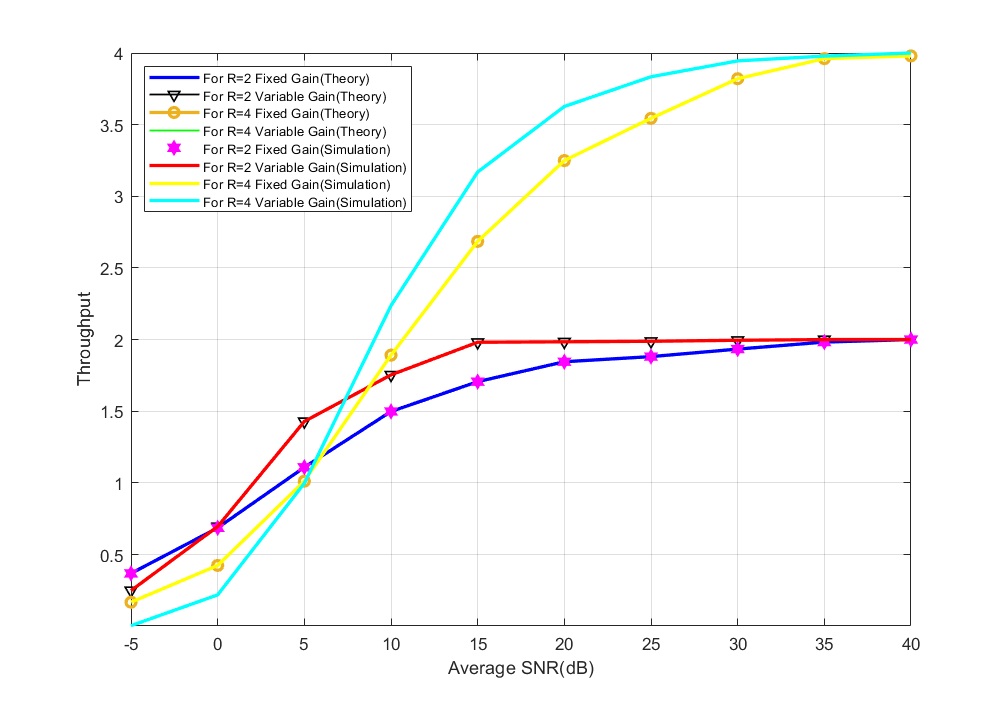
\includegraphics[width=\textwidth]{throughput.png}
    \caption{1R.}
  \end{minipage}
  \end{figure}
  \item Here, as shown above Fig 1B and 1R are graphs plotted of the Throughput versus Average SNR(dB). Parameters used which influences the figure, are
  \\1. The distance between the mobility nodes.
  \\2. Path loss component
  \\3. SIC Capability
  \\Thus, we find the Minimum required data rate (R) and eventually that leads us to calculating Throughput.
  \\As we consider 2 minimum required data rates, R=2 and R=4, we observe that during low SNR, the difference between the system throughput of the Double Rayleigh system and that of system over Rayleigh fading channel is significant.
\\Hence, the considered FD-V2V communication system cannot reach the required data rate, especially at high data transmission rate, i.e. R = 4 bit/s/Hz.
\end{itemize}

\subsection{New Results}
\begin{itemize}

\item New Result-1\\

\begin{center}
\includegraphics[height=6cm] {Transmitter_Relay.PNG}
\begin{figure}[h!]
  \caption{Transmitter Relay}
\label{fig:}
\end{figure}
\end{center}
\item INFERENCE OF NEW RESULT-1
\\In the above figure the results have been reproduced by calculating the outage probability of the fixed gain by comparing the channel coefficient with SNR threshold using SIMO system simulation model. It is inferred from this that by changing the system model from SISO to SIMO the system performance increases effectively.   
\end{itemize}

\begin{itemize}
\item New Result-2\\

\begin{center}
\includegraphics[height=6cm] {Relay_Receiver.PNG}
\begin{figure}[h!]
    \caption{Relay to Receiver}
\label{fig:}
\end{figure}
\end{center}
\item INFERENCE OF NEW RESULT-2
\\From the given above figure, signal transmitted from relay to receiver uses MISO system model. it is inferred that the system performance is considered significantly better than the SISO system model. Thus, on increasing the antennas on relay node the SNR improves and system model can be improved effectively.  

\end{itemize}

\begin{itemize}
\item New Result-3\\

\begin{center}
\includegraphics[height=6cm] {Combined.PNG}
\begin{figure}[h!]
  \caption{Combined}
\label{fig:}
\end{figure}
\end{center}
\item INFERENCE OF NEW RESULT-3
\\ In the above figure we have combined the results of SISO,MISO and SIMO system model from which we can justify and compare that when the Double Rayleigh Fading channel is compared with different system model it is inferred that that SIMO system model is comparatively better than the other two model whereas the MISO system model is better than the SISO system model considered in the base article.
\end{itemize}

\begin{itemize}
\item New Result-4\\
\begin{center}
\includegraphics[height=6cm] {NR1.PNG}
\begin{figure}[h!]
  \caption{The SER of the considered FD-V2V communication system using BPSK model with alpha=4 and gain=-30db}
  \item In the above figure results have been derived by keeping the distances between transmitter to relay and relay to destination same. It can be inferred that on decreasing the distance SER is decreased significantly and moreover by increasing the antennas on Relay node the performance metric can be improved significantly
\label{fig:}
\end{figure}
\end{center}
\end{itemize}

\begin{itemize}
\item New Result-5\\
\begin{center}
\includegraphics[height=6cm] {NR2.PNG}
\begin{figure}[h!]
  \caption{The impact of path loss exponent on the SER of the considered system for different path loss exponents}
  \item The above figure explains the effect of path loss exponent on our System Model. It can be inferred that in the loss signal strength will be very low if attenuation is decreased significantly. Moreover if we increase the antennas on relay node the signal which has received the least attenuation can be choose to transmit at receiver end.
\label{fig:}
\end{figure}
\end{center}
\end{itemize}


\begin{itemize}
\item New Result 6
\begin{center}
\includegraphics[height=6cm] {NR5.PNG}
\begin{figure}[h!]
  \caption{The SER of the considered system for different settings of the distances among vehicles}
  \item In the above figure results have been derived by keeping the distances between transmitter to relay and relay to destination different . It can be inferred that on decreasing the distance SER is decreased significantly and moreover by increasing the antennas on Relay node the performance metric can be improved significantly
\label{fig:}
\end{figure}
\end{center}
\end{itemize}

\begin{itemize}
\item New Result-7\\
\begin{center}
\includegraphics[height=6cm] {NR4.PNG}
\begin{figure}[h!]
  \caption{The SER of considered system for different average SNR'S}
  \item The above figure explains the effect of signal to noise ratio on System Model. On improving SNR performance metric is improved significantly. Moreoevr on increasing the antennas on relay node the SNR improves and system model can be improved
\label{fig:}
\end{figure}
\end{center}
\end{itemize}
	
\section{Conclusions}
	
\begin{itemize}


\item Derive conclusion-1 from the new work.Different scenarios had been considered such as for different path loss exponents, increasing SNR, changing distances between mobile node but none of them improved the system model significantly. However when the number of antennas were increased on the relay node and when a SIMO-MISO system was established the SER decreased significantly and the system model was improved. As the receiver gets multiple diversity it AF the signal with highest signal strength. Further research can be done to change the channel coefficients to improve the system model. 
\end{itemize} 


\begin{itemize}	
\item Derive conclusion-2  
\\ On comparing different models for increasing SNR and decreasing SER. The system performance while deriving the expression for outage probability we acknowledged that the SIMO-MISO system improved the system performance relatively. 
\end{itemize}

\section{ Contribution of team members}	
\subsection{Technical contribution of all team members }

\begin{table}[h]
\centering
\begin{tabular}{|l|l|l|l|l|}
\hline
\textbf{Tasks} & \textbf{Nimil} & \textbf{Aayushi} & \textbf{Priyanshi}& \textbf{Shashwat}\\ \hline
Task-1        & SER simulation                        & Throughput Simulation and Analytical                       & Outage Probability Simulation and Analytical                   & SER analytical   \\ \hline

Task-2         &  SER simulation for different parameters                      & OP Simulation for different parameters                       & OP Simulation for different parameters                    & SER analytical for different parameters  \\ \hline

Task-3         &  SER simulation for innovation                      & OP Simulation for innovation                       & OP Simulation for innovation                    &SER analytical for innovation
\\ \hline
\end{tabular}
\end{table}

\subsection{Non-Technical contribution of all team members }

\begin{table}[h]
\centering
\begin{tabular}{|l|l|l|l|l|}
\hline
\textbf{Tasks} & \textbf{Nimil} & \textbf{Aayushi} & \textbf{Priyanshi}& \textbf{Shashwat} \\ \hline
Task-1         &    Literature Survey                     &    Literature Survey                     &     Literature Survey                   &Literature Survey  \\ \hline
Task-2         &  Report Writing in Latex                      &Report Writing in Latex                        & Report Writing in Latex                      & Report Writing in Latex\\ \hline
 
\end{tabular}
\end{table}

\newpage

\item 
\begin{thebibliography}{9}
\bibitem{latexcompanion} 
David W. Matolak.
\textit{V2V Communication Channels: State of Knowledge, New Results, and What’s Next}. 
Department of Electrical EngineeringUniversity of South CarolinaColumbiaUSA.
 
\bibitem{einstein} 
Jihyung KimJunhwan LeeSangmi MoonIntae Hwang. 
\textit{A Position-based Resource Allocation Scheme for V2V Communication}
Wireless Transmission Research Section5G Giga Communication Research Laboratory, Electronics and Telecommunications Research Institute DaejeonRepublic of Korea.

\bibitem{latexcompanion} 
DongyaoJia Dong Ngoduy
\textit{Enhanced cooperative car-following traffic model with the combination of V2V and V2I communication}. 
Department of Electrical Engineering University of South Carolina Columbia USA.

\bibitem{latexcompanion} 
Tjiang
\textit{Channel modeling and inter-carrier interference analysis for V2V communication systems in frequency-dispersive channels}. 
	Department of Electronics and Information Engineering, Huazhong University of Science and Technology, Wuhan, China
	
	
\bibitem{latexcompanion}
Zhuorong Li,Hongyang Zhang
\textit{Vehicular ad hoc networks: architectures, research issues, methodologies, challenges, and trends}. 
	Department of Electronics and Information Engineering, Huazhong University of Science and Technology, Wuhan, China
	
\bibitem{latexcompanion}
M Khairnar, D Vaishali, DSN Pradhan 
\textit{V2V communication survey wireless technology}.Department of Electrical Engineering University of South Carolina Columbia USA.

\end{thebibliography}

\end{itemize}




%\bibliographystyle{IEEEtran}
%\bibliography{ref.bib}

\end{document} 